\documentclass[H:\workspace\担保人财务信息2\杭州大运河\HangZhouText.tex]{subfiles}
\begin{document}
\section{淮安市文旅游集团所做的关于大运河的项目}
\subsection{主营业务}
2020年3月,淮安市文化旅游集团股份有限公司(以下简称“公司”)揭牌成立,淮安文旅集团按照助力“绿色高地、
枢纽新城”发展定位,聚焦大运河文化带建设、全域旅游及文旅融合发展,
主营业务有餐饮酒店、旅游度假、实景娱乐、科普研学、赛事会展、文化创意、乡村振兴、物业地产“八大板块”。
\footnote{可以关注一下公司的股东,淮安新城投资开发有限公司,信用评级为 $\textcolor{red}{AA^{+}}$,
主营业务是基础设施、公共配套、社会事业以及民生保障项目的投资建设。}\par 

公司目前主要运营的项目有以下7个,
\begin{itemize}
    \item 里运河旅游;
    \item 白马湖旅游度假区;
    \item 板闸遗址公园;
    \item 中国漕运城;
    \item 水工科技馆;
    \item 滨河大道景观;
    \item 淮阴新华印刷厂;
\end{itemize}

其中,与大运河相关的项目主要有以下两个。
\begin{itemize}
    \item 里运河旅游,里运河文化长廊;
    \item 板闸遗址公园;
\end{itemize}

我们重点介绍下\uuline{里运河旅游项目}。
\subsection{里运河旅游项目}
\subsubsection{背景介绍}
在2021年1月举行的,淮安市第八届人民代表大会上,市长陈之常提出,要在全省率先出台大运河文化遗产保护条例,
成立大运河办、组建文旅集团,统筹推进大运河保护开发,启动中国水工科技馆等一批重大文旅项目,
同时要强力推进大运河沿岸化工企业整治、棚改拆迁攻坚扫尾、问题楼盘处置、省运河公司改制搬迁等难点工作。
\footnote{c.f. \href{http://www.hynews.net/p/122726.html}{政府工作报告}}

\subsubsection{业务模式}
淮安市里运河文化长廊是国家4A级旅游景区,贯穿淮安东西,全长32公里,主要由淮安新城投资开发有限公司负责。
景区内分布着清江浦记忆馆、淮安戏曲博物馆、淮安名人馆、
淮安市运河楹联馆、陈潘二公祠、吴公祠、斗姥宫、名人故居等景点,现已开通水上游船项目,游船自清江浦码头出发,
途经中洲岛、清江浦楼、榷关、河下古镇御码头、石板街、闻思寺等二十多处景点。
目前还开通了两条水上精品旅游线路:有以御码头为起始点,复走帝王南巡之路的“全程游”,游览时间1小时;
有以清江浦景区为中心的“市区游(夜景游)”,闸口游船码头出发,途经中洲岛、清江浦楼、越秀桥、
清江大闸、石码头桥、大运河文化广场、常盈桥、水门桥、长征桥,然后原路返回闸口游船码头,游览时间35分钟左右。
\footnote{c.f. \href{http://www.hactg.com/index.php?c=article&id=509}{介绍}}
票价如下。
\vspace{-1em}
\begin{table}[H]
    \centering 
    \xiaowuhao 
    \setlength{\tabcolsep}{1.2em} % for the horizontal padding
    {\renewcommand{\arraystretch}{0.5} % for the vertical padding 
    \begin{tabular}{@{}c|c|c@{}}
        \toprule[0.05cm]
        项目 & 成人票价 & 儿童票价 \\
        \midrule[0.025cm]
        全程游 & 80/人,往返100 & 40元/人,往返50 \\
        \midrule 
        市区游 & 50元/人 & 25元/人 \\
        \bottomrule 
    \end{tabular}
    }
    \caption{票价信息}
\end{table}

根据《淮安市里运河景观规划文本》,相关规划图如下 

\begin{figure}[H]
    \centering 
    \begin{subfigure}[t]{0.4\textwidth}
        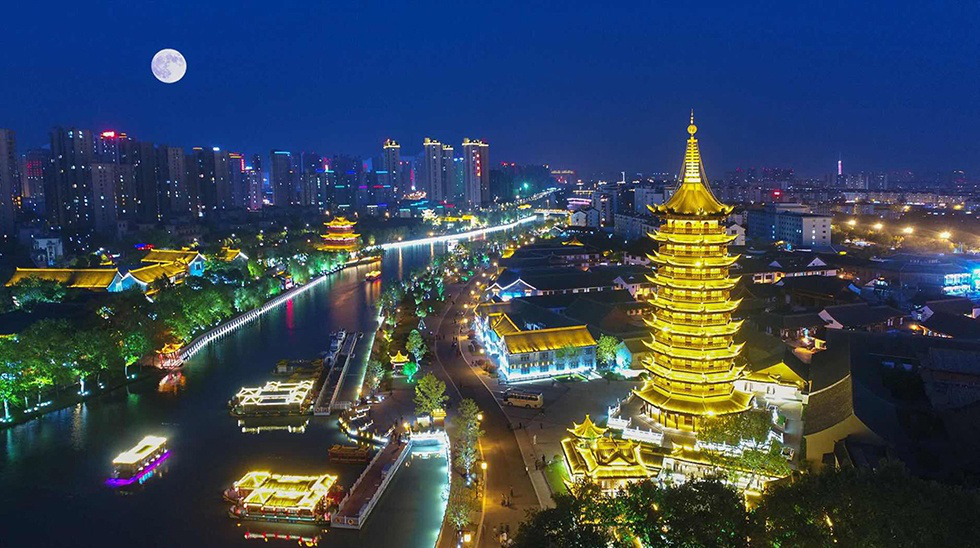
\includegraphics[width=\textwidth]{img8.png}
        \caption{效果图:1}
        \label{fig:1}
    \end{subfigure}
    \hfill 
    \begin{subfigure}[t]{0.4\textwidth}
        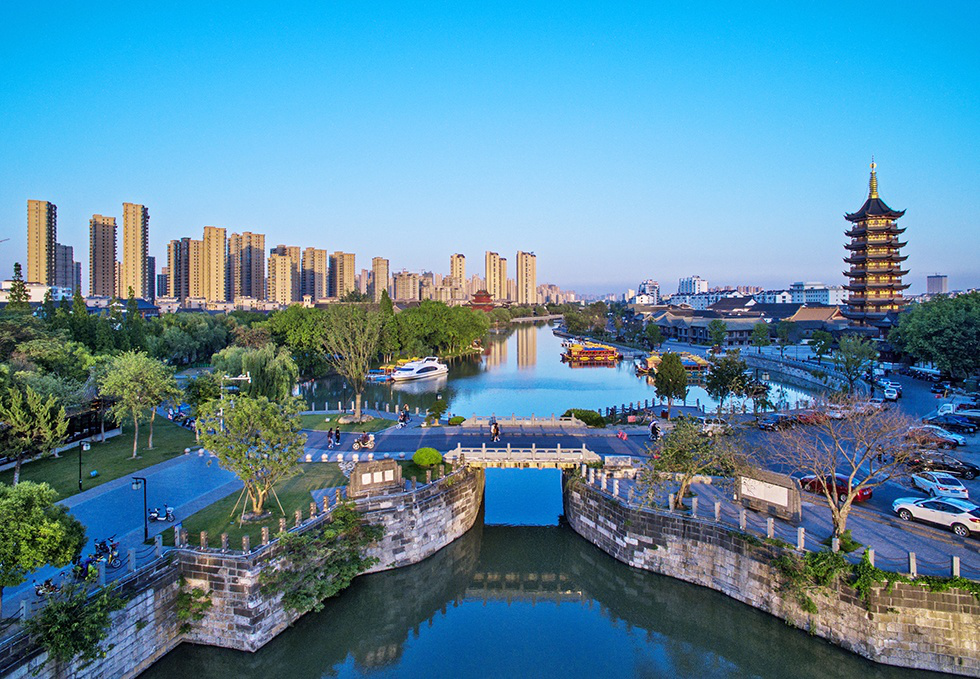
\includegraphics[width=\textwidth]{img9.png}
        \caption{效果图:2}
        \label{fig:2}
    \end{subfigure}
    \hfill 
    \begin{subfigure}[b]{0.4\textwidth}
        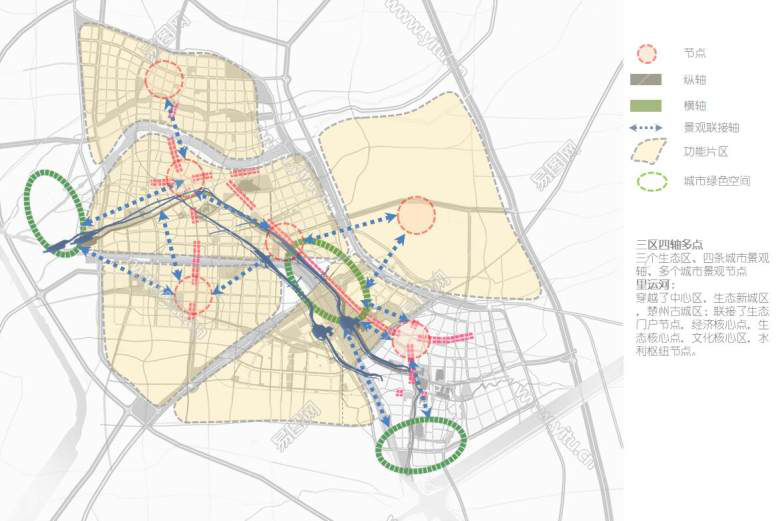
\includegraphics[width=\textwidth]{img10.png}
        \caption{效果图:3}
        \label{fig:3}
    \end{subfigure}
    \hfill 
    \begin{subfigure}[b]{0.4\textwidth}
        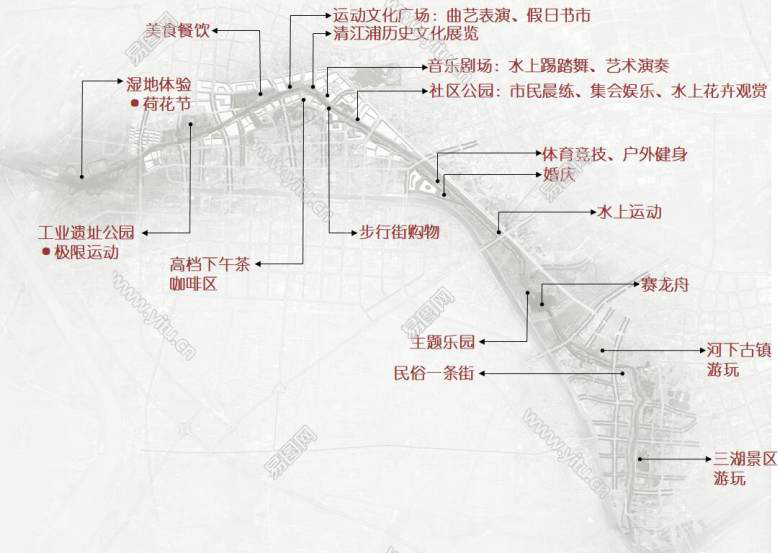
\includegraphics[width=\textwidth]{img11.png}
        \caption{效果图:4}
        \label{fig:4}
    \end{subfigure}
    \hfill 
    \begin{subfigure}{0.4\textwidth}
        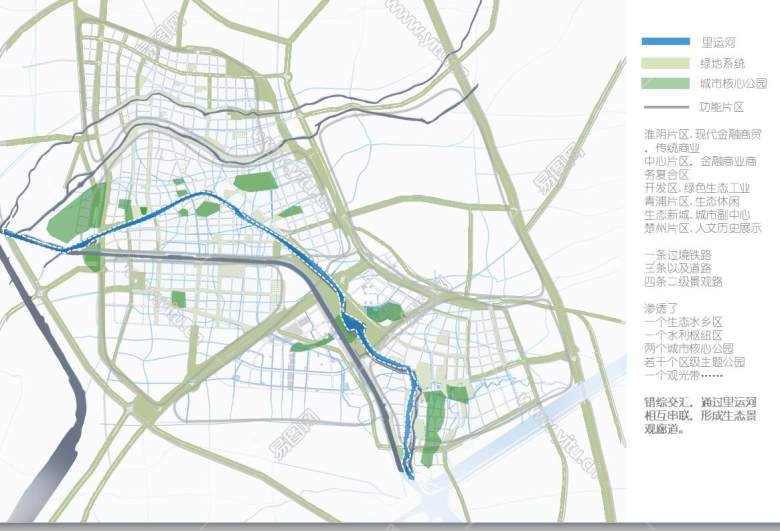
\includegraphics[width=\textwidth]{img12.png}
        \caption{效果图:5}
        \label{fig:5}
    \end{subfigure}

    \caption{里运河规划图}
    \label{fig:figure}
\end{figure}

\subsection{资金来源}
项目运营与维护的资金来源有三个,财政专项资金、自有资金和外部融资,业务模式采取委托代建模式。
对于外部融资,其中银行借款12次,共11.51亿;信托融资2次,共1.8亿;银行授信 14 次,共 21 亿。
主要合作企业有,常州丽景园林建设有限公司,主要负责里运河轮埠路(越秀桥-八亭桥)的人文自然景观及永久性绿地工程;
扬州市阳瑞电气工程有限公司,负责淮安里运河文化长廊景观亮化工程。
\end{document}